%
% TODO: Scrum
% Joel Spolsky
% https://www.joelonsoftware.com/2007/10/26/evidence-based-scheduling/
%
\newpage
%-------------------------------------------------------------------------
\chapter{Project Planning}
%
This chapter will cover methods how to control a project. Stakeholders
measure projects by how well they are executed within the project
constraints or baselines. A project baseline is an approved plan for a
portion of a project. It is used to compare actual performance to
planned performance and to determine if project performance is within
acceptable guidelines.\\
The following 4 project baselines should be considered:
\begin{itemize}
\item Quality
\item Schedule
\item Scope
\item Budget
\end{itemize}

Results:
\begin{itemize}
\item {\textbf Cost plan}: Creating budget / offer. %Ausarbeitung des Budgets resp. der Offerte
\item {\textbf Time plan}: Define activities, deadlines and milestones. %Festlegung der Aktivitäten, Termine und Meilensteine
\item {\textbf Employee plan}: Nomination of people and their working time. %Benennung der beteiligten Mitarbeiter/innen mit ihren Einsatzzeiten
\item {\textbf Organization plan}: Agreement of team structure, nomination of responsible persons. %Festlegung der Team-Struktur, Bezeichnung der Verantwortlichkeiten
\item {\textbf Quality plan}: Compilation of documents, tools and methods to ensure quality. %Zusammenstellung der Dokumente, Werkzeuge und Methoden zur Sicherstellung der Qualit\"at
\item {\textbf Project monitor plan}: Agreement of actions to control the project and if needed how to change the plans. %Festlegung der Massnahmen zur Kontrolle der Planeinhaltung, ggf. zur \"Anderung der Pl\"ane
\item {\textbf Configuration management plan}: Agreement of actions to control changes in documents, code or data (or any other resources). %Festlegung der Massnahmen zur Kontrolle der \"Anderungen in den Dokumenten, Programmen und Daten
\item {\textbf Education plan}: Definition of education for internal (project team) and external people (users, operating stuff). %Festlegung der internen (Mitarbeiter) und externen (Kunde, Anwender, Systembetreiber) projektspezifischen Ausbildung
\item {\textbf Risk management plan}: Agreement of actions to avoid or mitigate risks. %Festlegung der Massnahmen zur Vermeidung eines eventuellen Disasters.
\end{itemize}
\newpage
%--------------------------------------------------------------------------
\section{Classical/Traditional project planning}
\ifslides
\begin{center}
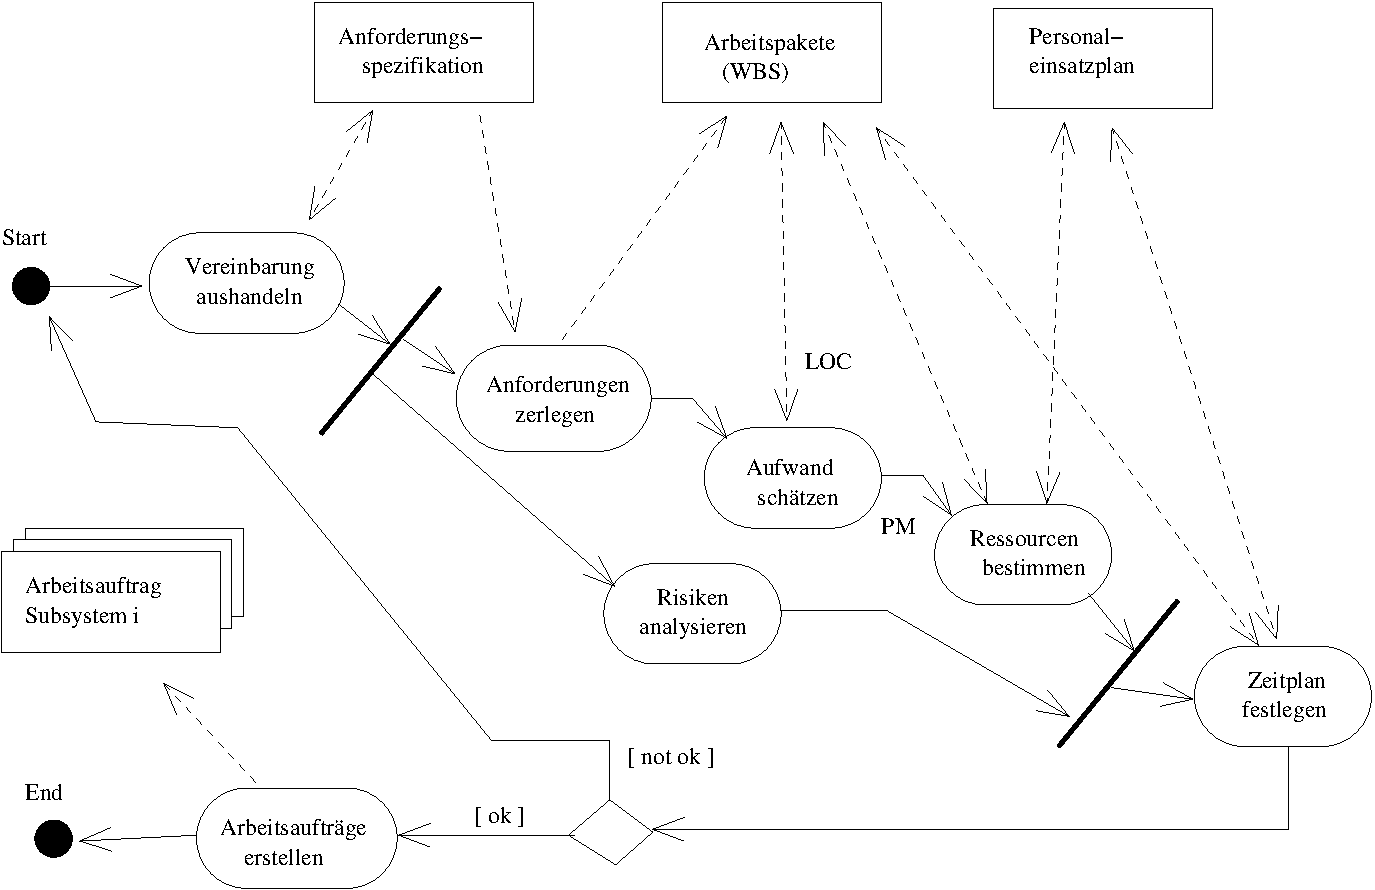
\includegraphics[width=0.85\linewidth]{lifecycle/xfig/planung}
\end{center}
\else
The process to create a project plan contains the following
activities:\\[3ex]
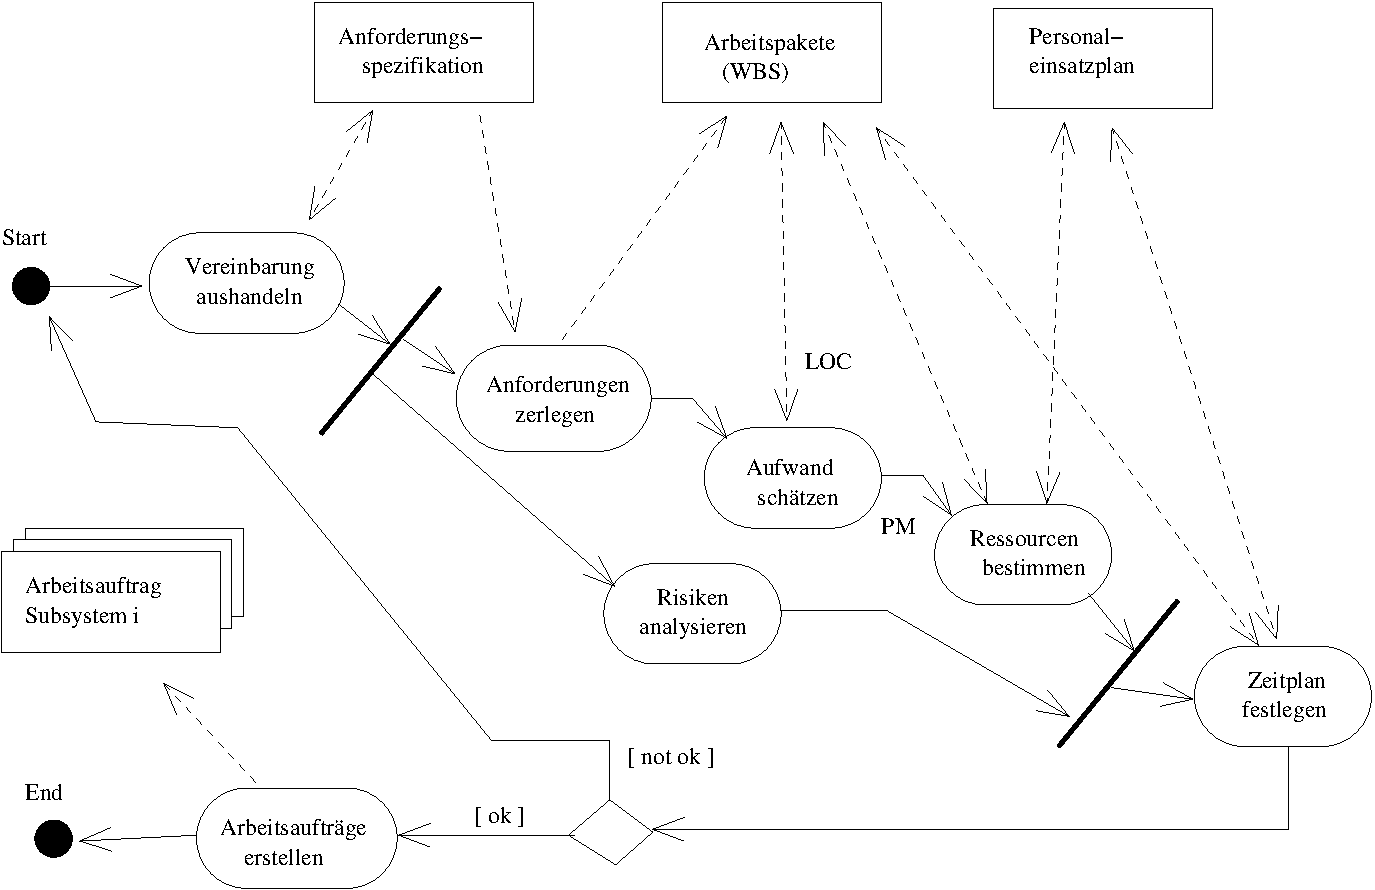
\includegraphics[width=\linewidth]{lifecycle/xfig/planung}\\[2ex]
\fi
\begin{enumerate}
\item \structure{Arrange agreement}:
  Define the project scope with a high level time schedule,
  point in time of devliverables, definition of mile stones.
  %Festlegung des Projektumfanges mit
  %einer groben Terminplanung, Abgabezeitpunkte der Liefergegenstände,
  %(engl. deliverables), Definition der Meilensteine
\item \structure{Breakdown requirements}:
  Breakdown the requirements into work packages according to the defined
  deliverables, create WBS (work breakdown structure). Recommended time
  for one work package is 4-6 weeks.
  %an den Liefergegenständen orientierte Zerlegung
  %in ``handhabbare'' Arbeitspakete, Aufstellung des Projektstrukturplans
  %(engl. Work breakdown structure WBS), empfehlenswerte Grössenordnung: 4-6
  %Wochen Zeitdauer pro Arbeitspaket,
\item \structure{Estimate effort}:
  Estimate effort for each package based on a value which could be measured.
  For software components, this could be LOC (lines of code). The LOC value
  could be used to get the amount of time needed for that component.
  %am besten auf Basis einer
  %(messbaren) Grössenschätzung für einzelne Arbeitspakete, bei SW-Komponenten
  %z.B: Lines of Code (LOC), daraus kann mittels
  %Erfahrungswerten der Aufwand in Personenmonaten (PM) bestimmt
  %werden,
\newslide
\item \structure{Define resources}:
  Assign people to activities with respect of their
  availability, qualification (education) and demand.
  The best way to do that is the usage of a model with
  roles and responsibilities.
  %Zuordnung der Personen zu den Aktivitäten
  %entsprechend des Bedarfes, ihrer Qualifikationen und Verfügbarkeit,
  %idealerweise auf Basis von Rollen und Verantwortlichkeiten
\item \structure{Analyse risks}:
  Identify and prioritize potential risks and possible actions.
  %Identifikation/Priorisierung der potentiellen
  %Probleme und möglicher Gegenmassnahmen
\item \structure{Define schedule}:
  Description of all work packages and their time dependencies.
  When is the final point in time to deliver a package, are there any
  dependencies to other packages? This is typically done with a
  gantt chart or network diagram.
  %Beschreibung/Darstellung der terminlichen
  %Rahmenbedingungen der
  %Aktivitäten sowie ihrer gegenseitige Abhängigkeiten (z.B. durch
  %Tabellen, Netzplantechnik, Ganttdiagramme) unter Berücksichtigung der Risiken
\end{enumerate}
\newpage
%-------------------------------------------------------------------
\section{Agile project planning}
Software development is a constant dialog between \emph{What is possible} and
\emph{What is needed}.
%
\begin{itemize}
\item \structure{Planning}: only plan for the next
  iteration, version. Not more!
\item \structure{Responsibility} will be taken over, not assigned
\item \structure{Estimates}: the responsible persons define the effort and duration
\item \structure{Priorities} define the order,
\end{itemize}

\newslide
The business side (Product Owner) decides
\begin{itemize}
\item \structure{MVP}: Minimal viable product. How should the problem be solved to
bring additional value. What is to much, what is not enough?
\item \structure{Priority}: Which tasks should be executed first?
\item \structure{Release}: Which pieces should be part in the next release?
\item \structure{Delivery}: Which timeframe is available to be successful?
\end{itemize}

\newslide
The developers have the freedom to take over responsibility and decide for
\begin{itemize}
\item \structure{Effort}: how long will it take to implement a specific feature?
\item \structure{Consequences}: what are the consequences for a taken approach?
\item \structure{Process}: what is the structure for the work and the team?
\item \structure{Planning}: when will the features be delivered
\end{itemize}

%
\newpage
\subsection{Cost Estimation}
The total costs of software projects contains
%Die Totalkosten einer Software-Entwicklung setzen sich zusammen aus:
\begin{itemize}
\item {\textbf Software-Cost}: software, licenses
\item {\textbf Hardware-Cost}: infrastructure (own hardware, cloud-based systems)
\item {\textbf Personal-Cost}: Salary, Expenses
\end{itemize}
\ifslides
\newpage
\fi
Precision of the cost estimation:
\ifslides
\begin{center}
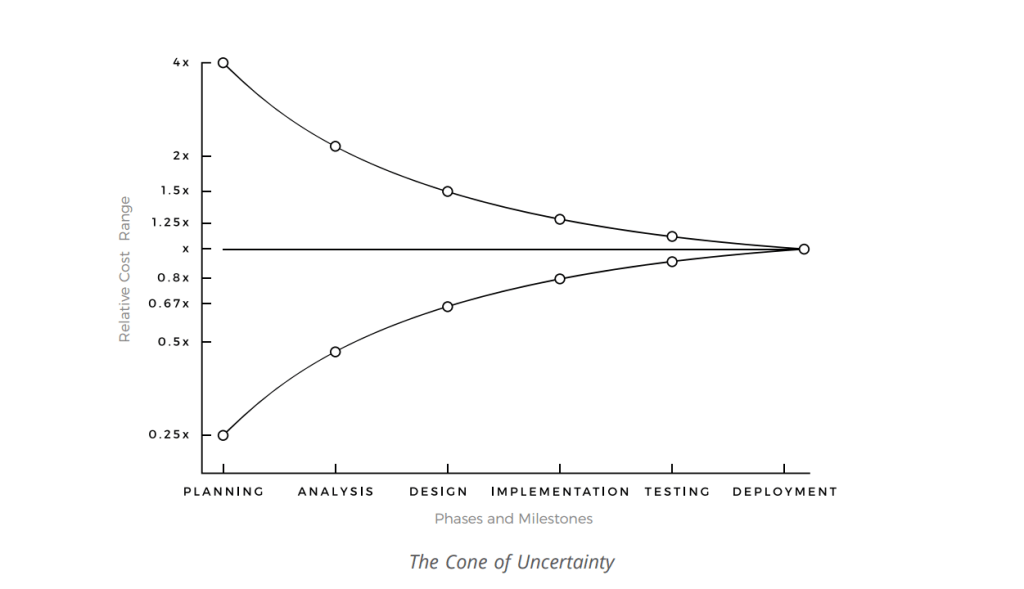
\includegraphics[width=0.75\linewidth]{lifecycle/img/cost_estimates}\\[2ex]
\end{center}
\else
\\[2ex]
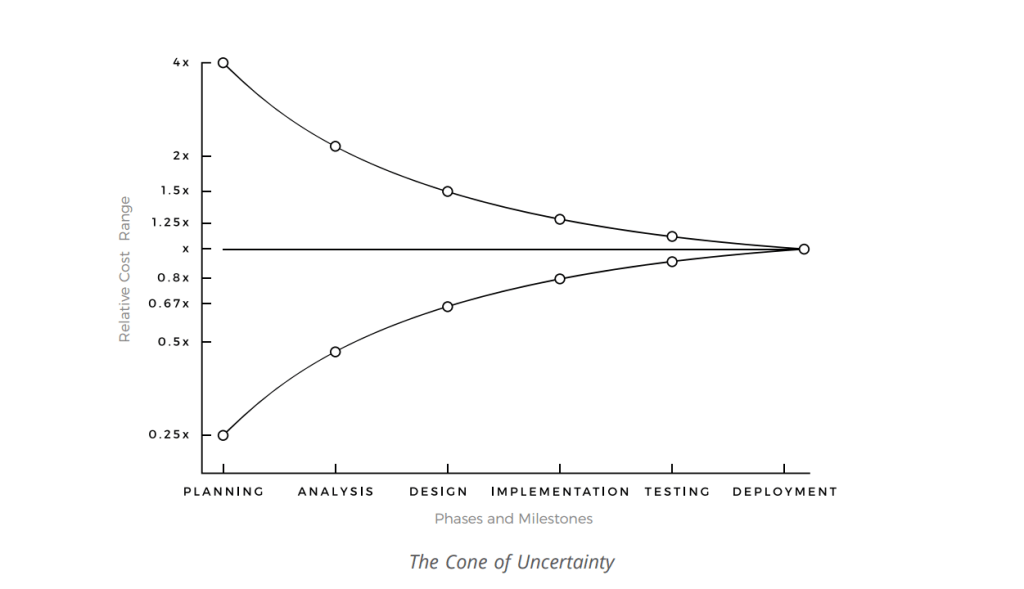
\includegraphics[width=1.0\linewidth]{lifecycle/img/cost_estimates}\\[2ex]
\fi
%
Influencing factors to estimate the costs:
\begin{itemize}
\item {\textbf Size}: Lines of code, classes, methods
\item {\textbf Complexity}: Dependency between the modules, is it possible to build modules?, HW/SW environment
\item {\textbf Experience}: Number of similar executed projects
\item {\textbf Reliability}: error rate, system stability
\end{itemize}
\newpage
There are several methods to estimate the costs:
\begin{itemize}
\item Empiric estimation methods:
\begin{itemize}
\item {\bfseries Expert judgment:}
  Several experts on the proposed software development techniques and
  the application domain are consulted. They each estimate the project
  cost. These estimates are compared and discussed. The estimation
  process iterates until an agreed estimate is reached.
  %Vergleich mit durchgeführten Projekten mittels
  %direkter Analogieschätzung, Schätzung durch Zerlegung in Teilaufgaben,
  %Drei-Punkt-Schätzung (optimistisch, realistisch, pessimistisch),
\item {\bfseries Delphi method:}
  Delphi technique is quite an old but efficient forecasting method.
  It follows an interactive approach which relies on exchange of ideas.
  The team is composed of a group of experts in their respective domains,
  who answers the queries in two or more rounds. Every time a facilitator
  provides a summary of the collected ideas, which is revised by the
  experts if required. The process of opinion and revaluation goes on
  until a final consensus is reached.\\
  Delphi technique relies its assumption on the fact that assimilation
  of ideas from a structured group leads to a productive outcome.
  %mehrere Experten geben unabhängig voneinander
  %eine Schätzung ab, anschliessend wird der Mittelwert bekannt gegeben und das
  %Verfahren solange wiederholt, bis alle Schätzungen einigermassen bei
  %einander liegen,
\end{itemize}
\ifslides
\newpage
\fi
\item Algoritmic estimation methods:
\begin{itemize}
\item {\bfseries Function Point Analysis:}
  Function Point Analysis is a standardized method used commonly as
  an estimation technique in software engineering.\\
  In simple words, FPA is a technique used to measure software
  requirements based on the different functions that the requirement
  can be split into. Each function is assigned with some points based
  on the FPA rules and then these points are summarized using
  the FPA formula. The final figure shows the total man-hours
  required to achieve the complete requirement.
  %Zählung und Gewichtung der Funktionen unter
  %Berücksichtigung
  %der Schnittstellen, Eingaben, Ausgaben, Umformungen, Abfragen und
  %Datenbestände,
  %nicht geeignet für Programme mit hoher algorithmischer Komplexität und/oder
  %komplexer Benutzerschnittstelle, kaum messbar
\item {\bfseries Widget Point Analysis:}
  Count the UI (user interface) elements and calculate out of this
  number the function points. Only useful for software with user interfaces and
  not many algorithmic calculations in the background.
  %Zählung der User-Interface-Elemente und daraus
  %Ermittlung
  %der Funktionspunkte, nur für GUI-Programme mit geringer algorithmischer
  %Komplexität geeignet, leichte Reproduzier- und Messbarkeit
\item {\bfseries Lines of Code (LOC):}
  Easy measurement method. Dependent on the programming language and the
  available libraries.
  %einfache Messbarkeit jedoch abhängig von der
  %Programmiersprache
  %und der verwendeten Bibliotheken (libraries), kann im Verlauf eines
  %Projektes stark schwanken
\end{itemize}
\ifslides
\newpage
\fi
\item Other methods:
  \begin{itemize}
  \item {\bfseries Pricing to win }:
  The software cost is estimated to be whatever the customer has
  available to spend on the project. The estimated effort depends on the
  customer's budget and not on the software functionality.
  \item {\bfseries Pain threshold method}:
  Highest price which the customer is willing to pay
  %Soviel, wie der Auftraggeber gerade noch
  %bereit ist zu zahlen.
\item {\bfseries Parkinson's Law}:
Parkinson's Law states that work expands to fill the time available. The
cost is determined by available resources rather than by objective
assessment. If the software has to be delivered in 12 months and 5
people are available, the effort required is estimated to be 60 personmonths.
  \end{itemize}
\end{itemize}
\ifslides
\newpage
\fi
\underline{Function point analysis} (A.J. Albrecht)
Function points are used to compute a functional size measurement
(FSM) of software.: (\href{http://www.ifpug.org}{www.ifpug.org})
%Weitere Informationen: International Function Point User Group
\begin{center}
\begin{tabular}{|l|l|l|l|}
\hline
Category & Number & Value (low) average (high) & Total \\
\hline
External inputs & &  x (3) 4 (6) & \\
External outputs & & x (4) 5 (7) & \\
External inquiries & & x (3) 4 (6) & \\
Internal logical files & & x (7) 10 (15) & \\
External interface files & & x (5) 7 (10) & \\
\hline
\multicolumn{3}{|l|}{Total}  &\\
\hline
\end{tabular}
\end{center}
In a second step, the calculated function points could be converted into
LOC (lines of code):
%Ein Nachteil dieses Verfahrens ist, dass Function-Points nicht
%gemessen werden können. Albrecht schlägt deshalb vor, aus dem erhaltenen Wert
%in einem zweiten Schritt die Anzahl der
%Programmzeilen zu bestimmen.
\begin{center}
\begin{tabular}{|l|c|}
\hline
Programming language & LOC per FP \\
\hline
Assembler & 320 \\
C         & 128 \\
Fortran   & 128 \\
Pascal    & 91 \\
%Modula 2  & 80 \\
C++/Java  & 53 \\
SQL       & 13 \\
\hline
\end{tabular}
\end{center}
Attention: this method does not reflect the re-usage of software
components!
%Achtung:  bei dieser Methode wird die Wiederverwendung von
%Softwarekomponenten nicht berücksichtigt.

\vspace{5mm}

\newslide
%-------------------------------------------------------------------------------
%\subsection*{Kostensch\"atzung}
\underline{Widget point analysis} (H. Krasemann)\\[2ex]
Calculate the number of function points based on the elements of the
user interface.
%Aus der Anzahl der Elemente der Benutzeroberfläche die Funktionspunkte bestimmen:
\begin{equation}
 function points = 2\cdot widget points
\end{equation}
\begin{itemize}
\item {\bfseries Input widgets:} Textfield, Combobox, Menubutton, Radiobutton, Pushbutton,
  Checkbox
\item {\bfseries Describing widgets:} Label, Separator, Group box, Window
\item {\bfseries Composite widgets:} Notebook, Table, Scrollbar, List
\item {\bfseries Menu widgets:} Menu bars, Men items
\end{itemize}

\newslide
Example:%\\[3ex]

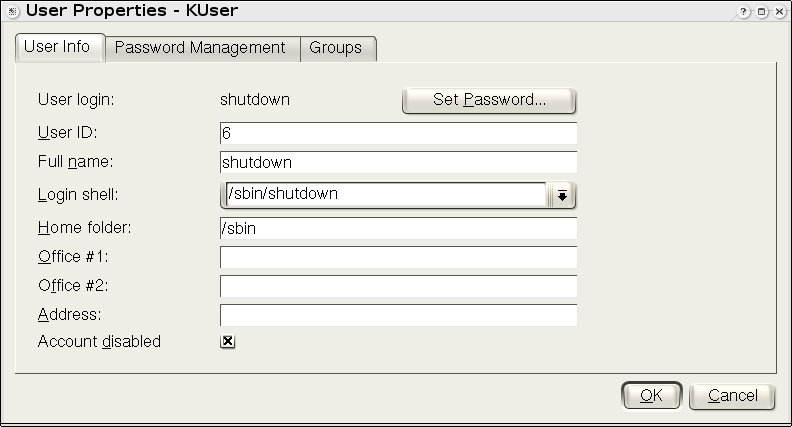
\includegraphics[width=\linewidth]{lifecycle/img/kuser}
%Beispiel:\\[2ex]
%\begin{tabular}{lr}
%Eingabewidgets & 9\\
%Beschreibende Widgets & 17 \\
%Zusammengesetzte Widgets & 1 \\
%\hline
%TOTAL  Widgetpunkte           & 27 \\
%TOTAL  Funktionspunkte           & 54 \\
%TOTAL LOC (C++)            & 2862 \\
%\end{tabular}
\newpage
%-------------------------------------------------------------------
%\section*{Projektplanung}
%\subsection*{Kostensch\"atzung}
\underline{COCOMO} (COnstructive-COst-MOdel, B. Boehm)
\begin{enumerate}
\item Calculation of the effort in person month:
\begin{equation}
 E_i = a \cdot KDL^b
\end{equation}
with the factor $a$\, the exponent $b$\
and $KDL$ as number of delivered lines of code (in thousand)
(Kilo-delivered-lines).\vspace{0.8cm}\\
\begin{tabular}{|l|cc|}\hline
Project type & a & b \\ \hline
organic (simple) & 3.2 & 1.05 \\
semi-detached (medium) & 3.0 & 1.12 \\
embedded (complex) & 2.8 & 1.20 \\ \hline
\end{tabular}\vspace{0.8cm}\\
\item Calculation of the effort in person month:
\begin{equation}
E = EAF \cdot E_i
\end{equation}
with the correction factor $EAF$ (Effort-adjustement-factor).
\end{enumerate}
\newpage
%--------------------------------------------------------------------------
\begin{enumerate}\setcounter{enumi}{2}
\item Possible correction factors $EAF$ from the table:
\ifslides
\\{\footnotesize
\else
\\[1.5ex]
\fi
\begin{tabular}{|lccccc|}\hline
Kostenfaktoren & very low & low & nominal & high & very high \\
        \hline & & & & &\\
Required Software Reliability & 0.75 & 0.88 & 1.00 & 1.15 & 1.40  \\
Size of Application Database &  & 0.94 & 1.00 & 1.08 & 1.16  \\
Complexity of The Product & 0.70 & 0.85 & 1.00 & 1.15 & 1.30  \\
Runtime Performance Constraints & & & 1.00 & 1.11 & 1.30 \\
Memory Constraints & & & 1.00 & 1.06 & 1.21\\
Response times & & 0.87 & 1.00 & 1.07 & 1.15 \\
Analyst capability & 1.46 & 1.19 & 1.00 & 0.86 & 0.71 \\
Applications experience & 1.29 & 1.13 & 1.00 & 0.91 & 0.82 \\
Software engineer capability & 1.42 & 1.17 & 1.00 & 0.86 & 0.70 \\
Programming language experience & 1.14 & 1.07 & 1.00 & 0.95 & \\
Application of software engineering methods & 1.24 & 1.10 & 1.00 & 0.91 & 0.82 \\
Use of software tools & 1.24 & 1.10 & 1.00 & 0.91 & 0.83 \\
Required development schedule & 1.23 & 1.08 & 1.00 & 1.04 & 1.10 \\
\hline
\end{tabular}
\ifslides
}
\fi
\vspace{0.8cm}\\
\item Calculation of the effort distribution (in percentage):
\vspace{0.8cm}\\
\begin{tabular}{|lccc|}\hline
Software size & small (2 KDL) & medium (32 KDL) & large (128 KDL) \\ \hline
 & & & \\
Design & 16 & 16 & 16 \\
Implementation & 68 & 62 & 59 \\
Integration + Tests & 16 & 22 & 25 \\ \hline
\end{tabular}
\end{enumerate}
\newpage
\underline{Story point method}\\
Story points are a unit of measure for expressing an estimate of
the overall effort that will be required to fully implement a
product backlog item or any other piece of work. When we
estimate with story points, we assign a point value to each item.
The raw values we assign are unimportant.\\

\vspace{3mm}

The Fibonacci sequence is one popular scoring scale for estimating agile
story points. In this sequence, each number is the sum of the
previous two in the series.\\

%In Scrum-Projekten werden \structure{Story Points}
%zur Bestimmung des Aufwands verwendet. Im Unterschied zu Zeiteinheiten
%bezeichnen Story Points die relative
%Grösse einer User Story. Von Mike Cohn stammt der Vorschlag dazu die
%Fibonacci-Reihe zu verwenden:

{\Large\centering
0, 1, 2, 3, 5, 8, 13, 21\ldots.
}

\vspace{3mm}

Also, it’s useful to set a maximum limit (13, for instance).
If a task is estimated to be greater than that limit, it should
be split into smaller items. Similarly, if a task is smaller than 1,
it should be incorporated into another task.\\

\vspace{3mm}

Before each estimation round, set 2 reference points:
two good predictable stories, one with 2 the other one with 5 points.\\

\vspace{3mm}

%Man sollte sich auf das Intervall 0 bis 8 beschränken und nur
%in Ausnahmefällen grössere Werte einsetzen.

%Zu Beginn einer Schätzrunde empfiehlt es sich zwei Referenzpunkte zu
%setzen: eine gut abschätzbare Story mit 2 und eine solche mit 5
%Punkten.
\newslide

A burndown chart shows the amount of work that has been
completed in an epic or sprint, and the total work remaining.
Burndown charts are used to predict your team's likelihood of
completing their work in the time available.
%vs. time. The outstanding work (or backlog) is often on the vertical
%axis, with time along the horizontal. It is useful for predicting when
%all of the work will be completed.:
\begin{figure}[H]
\centering
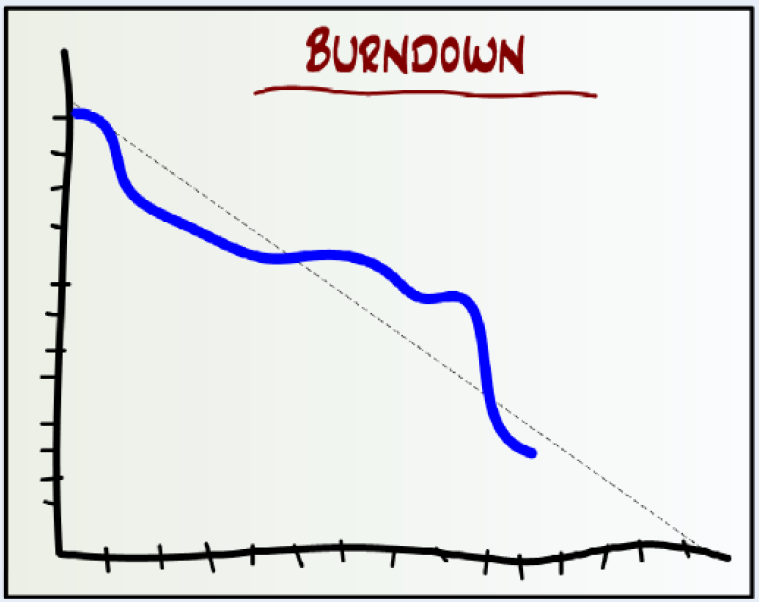
\includegraphics[width=0.55\linewidth]{lifecycle/img/burndownchart}
\caption{Burndown chart (Source: Henrik Kniberg)}
%\caption{Release Burndown Chart showing scope changes
%(Source http://alistair.cockburn.us/)}
\end{figure}
\newslide
% https://www.joelonsoftware.com/2007/10/26/evidence-based-scheduling/
%
And what about Microsoft Project?
Software development guru Joel Spolsky puts it this way:
\begin{quote}
"The trouble with Microsoft Project is that it assumes that you want
to spend a lot of time worrying about dependencies... I've found that
with software, the dependencies are so obvious that it's just not
worth the effort to formally keep track of them."
\end{quote}
Joel continues:
\begin{quote}
Another problem with Project is that it assumes that you're going to
want to be able to press a little button and ''rebalance'' the
schedule... For software, this just doesn't make sense [in
practice]... The bottom line is that Project is designed for building
office buildings, not software.
\end{quote}
Joel is a former Microsoft employee, who worked on both Excel and
Project.  He's not alone in his views. Chris Peters, Microsoft's Vice
President in charge of Office, also said that Microsoft Project is
more appropriate for managing the design of airplanes and buildings,
rather than
software. (\href{http://www.agilekiwi.com/earnedvalue/agile-charts}
{www.agilekiwi.com/earnedvalue/agile-charts})
%
\begin{itemize}
\item Aufwandschätzung mit Story Points (Mike Cohn)
\href{http://www.planningpoker.com/detail.html}
{www.planningpoker.com/detail.html}
\item How to implement Scrum:

\href{http://www.agile-software-development.com/2007/09/how-to-implement-scrum-in-10-easy-steps_20.html}{www.agile-software-development.com/2007/09/how-to-implement-scrum-in-10-easy-steps\_20.html}
\end{itemize}
%
\newpage
%--------------------------------------------------------------------------
%\section*{Projektplanung}
\section{Timeplan}
Axiom: Personen und Monate sind nicht austauschbar.
\begin{enumerate}
\item Calculate the length of a project in months based on the calculated
person months:
\begin{equation}
 D = 2.5 \cdot E ^{\;0.38}
\end{equation}
\item Caclculate the average demand of employees:
\begin{equation}
 P = \frac{E}{D}
\end{equation}
\ifslides
\newpage
\fi
\item Calculation of the effort distribution (in percentage)::\\[1.5ex]
\begin{tabular}{|lccc|}\hline
Software size & small (2 KDL) & medium (32 KDL) & large (128 KDL)\\ \hline
 & & & \\
Design & 19 & 19 & 19 \\
Implementation & 63 & 55 & 51 \\
Integration + Tests & 18 & 26 & 30 \\ \hline
\end{tabular}
\ifslides
\newpage
\fi
\item Refinement of all phases and creation of the predecessor list:
\begin{center}
\begin{tabular}{|l|l|c|c|l|}
\hline
No & Task & Predecessor & Duration & Ressource \\
\hline
1   & Software design &    & 5  & Meier \\
2   & Design approval & 1 & 1 & (Review) \\
3   & Implementation GUI & 2 & 25 & Hilfiker \\
4   & Implementation DB  & 2 & 12 & \ldots   \\
5   & Module test GUI &    3 & 3 & \ldots \\
6   & Module test DB  &    4 & 2 & \ldots \\
7   & Integration   &    5,6 & 2 & \ldots \\
\hline
\end{tabular}
\end{center}
\end{enumerate}

Further development of the model:

\href{http://sunset.usc.edu/csse/research/COCOMOII/cocomo_main.html}
  {sunset.usc.edu/csse/research/COCOMOII/cocomo\_main.html}

\newslide
Calculation software:
\begin{itemize}
\item  COCOMO 81 Intermediate Model Implementation:

  \href{http://sunset.usc.edu/research/COCOMOII/cocomo81_pgm/cocomo81.html}
  {sunset.usc.edu/research/COCOMOII/cocomo81\_pgm/cocomo81.html}

\item COCOMO II with Heuristic Risk Assessment:

  \href{http://sunset.usc.edu/research/COCOMOII/expert_cocomo/expert_cocomo2000.html}{sunset.usc.edu/research/COCOMOII/expert\_cocomo/expert\_cocomo2000.html}
\end{itemize}
\newpage
%------------------------------------------------------------------------------
\subsection{Critical Path Method / Critical Path Analysis}
The critical path method (CPM), or critical path analysis (CPA),
is an algorithm for scheduling a set of project activities.
It is commonly used in conjunction with the program evaluation and
review technique (PERT). A critical path is determined by identifying
the longest stretch of dependent activities and measuring the time
required to complete them from start to finish.\\

\vspace{4mm}

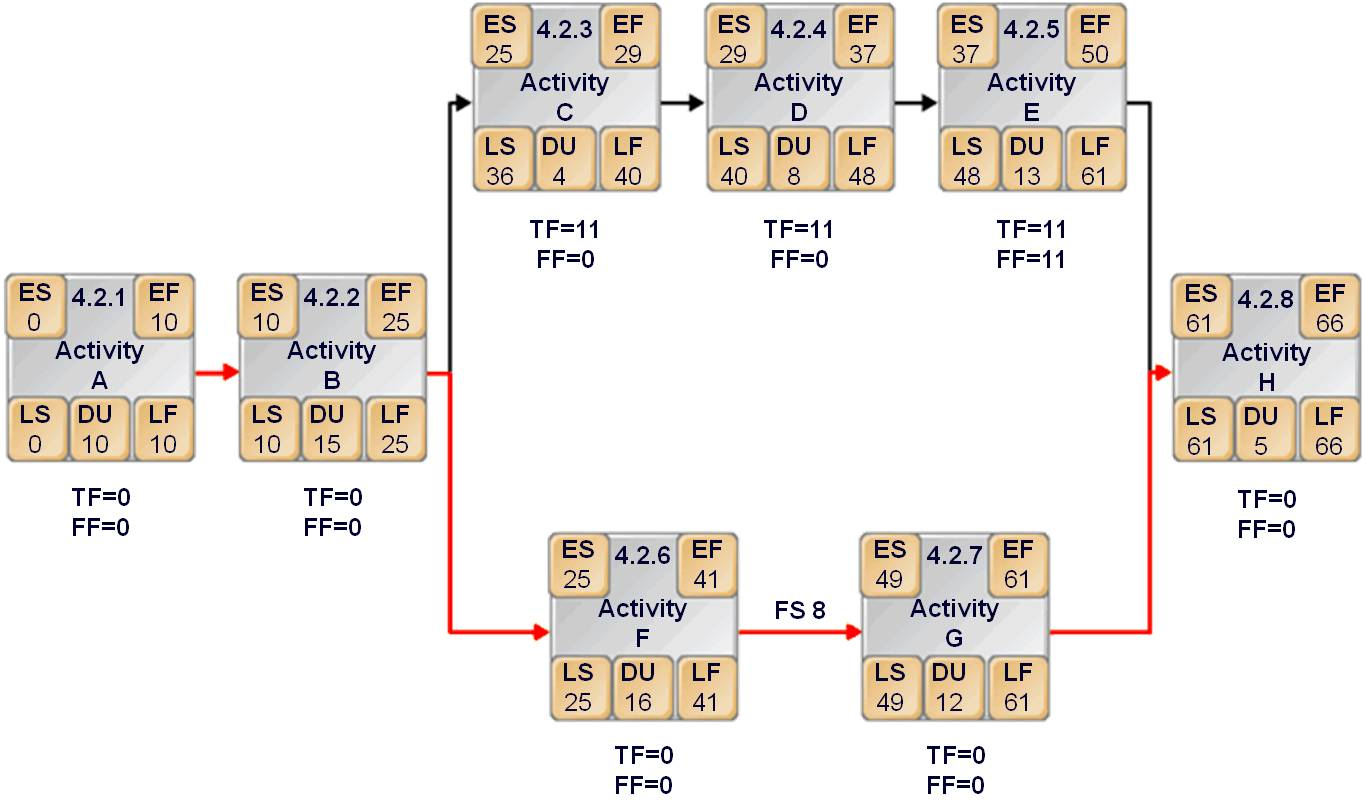
\includegraphics[width=1.0\linewidth]{lifecycle/img/networkdiagram}
%
\newslide
\newpage

\subsection{Gantt charts}
A Gantt chart, or harmonogram, is a type of bar chart that illustrates
a project schedule. This chart lists the tasks to be performed on the
vertical axis, and time intervals on the horizontal axis. The width
of the horizontal bars in the graph shows the duration of each
activity. Gantt charts illustrate the start and finish dates of the
terminal elements and summary elements of a project. Terminal elements
and summary elements constitute the work breakdown structure of the
project. Modern Gantt charts also show the dependency
relationships between activities. (wikipedia.org)
\ifslides
\begin{center}
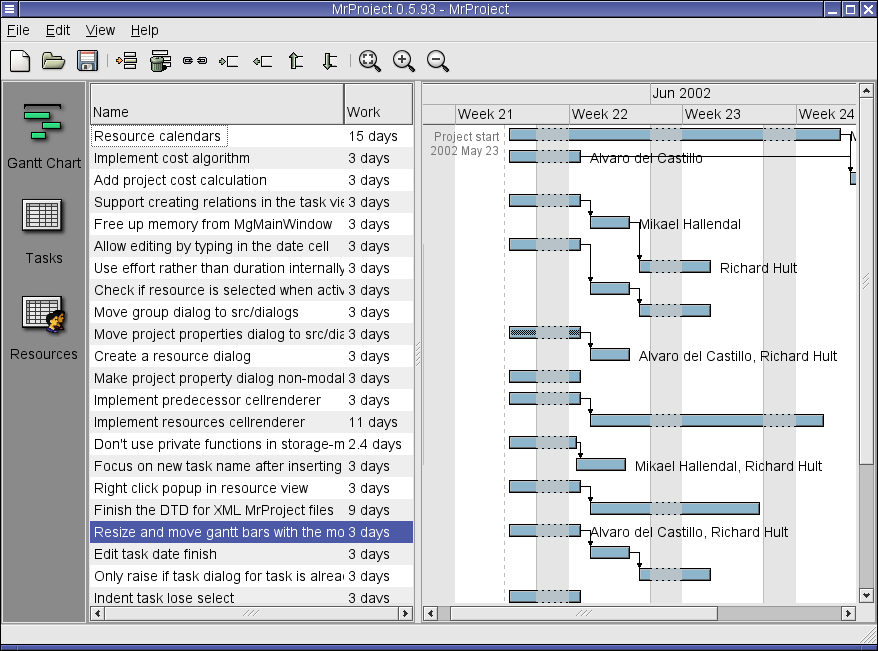
\includegraphics[width=0.75\linewidth]{lifecycle/img/mrproject-gantt}
\end{center}
\else
\vspace{0.5cm}
\begin{figure}[H]
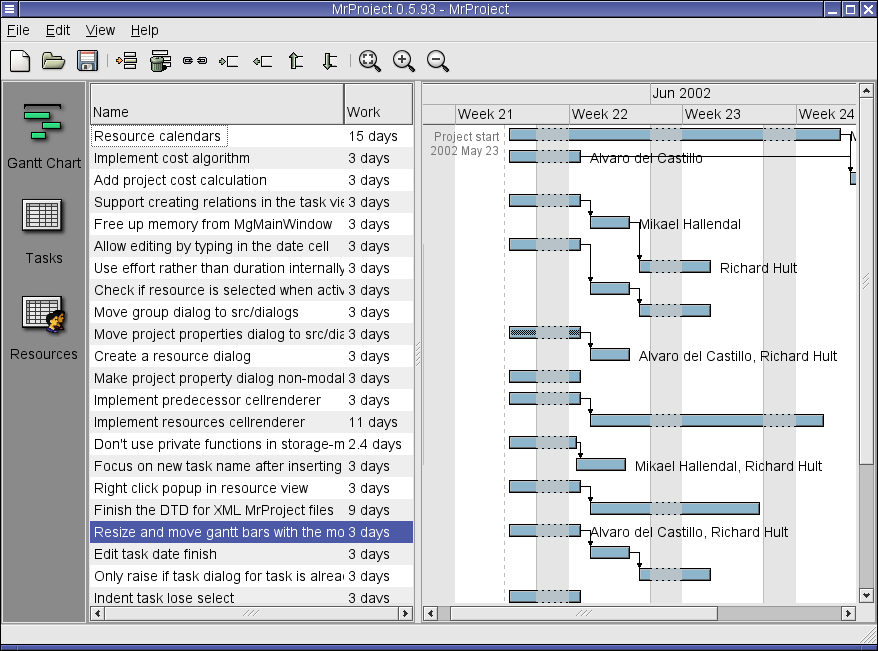
\includegraphics[width=\linewidth]{lifecycle/img/mrproject-gantt}
\caption{Source: \href{http://live.gnome.org/Planner}
               {live.gnome.org/Planner}}
\end{figure}
\fi
%Die Länge der Balken entspricht der Zeitdauer einer Aktivität.

%Bei der Erstellung eines Gantt-Diagrammes ist auf einen sinnvollen
%Detaillierungsgrad zu achten.
\newpage
%------------------------------------------------------------------------------
%\section*{Projektplanung}
\section{Risk Management}
Recognize, analyse and control risks:
%Risiken rechtzeitig erkennen, bewerten und kontrollieren können:
\ifslides
\\{\footnotesize
\else
\\[2ex]
\fi
\begin{tabular}{|l|p{8.5cm}|}
\hline
Risk & Reason \\
\hline
Change of requirements & Scope variations occur when the scope of an iteration
  changes after a timeframe had been agreed upon. Due to the value from
  receiving frequent customer feedback, stakeholders or product owners
  will often ask to vary the scope of a project\\
\hline
Unrealistic planning & Inaccurate estimations occur when the length of a
  project, milestone or iteration is underestimated by the project group.
  Software estimations can cause problems between developers and clients
  because they lead to increase project timeframes, and therefore also
  project expenses. There could also be a problem if people are not
  available due to job change, illness, accident or other reasons.\\
\hline
Missing experience & first usage of a technology, method, tools,
  reduced knowledge of the project area,
  complex SW/HW environment, special requirements, big data,
  high reliability\\
\hline
Improper infrastructure & instable or non-working HW/SW components. Problem with
  component delivery by 3rd party vendor\\
\hline
Financial issue      & Reorganization, incorrect budget estimation,
  project scope expansion, cost overruns\\
\hline
Communication issues & Inadequate support, misunderstanding, conflicts\\
\hline
\end{tabular}
\ifslides
}
\fi
\vspace{0.5cm}

Level of risk:
\begin{equation}
  Risk = Likelihood \cdot Severity
\end{equation}
Project management standards dictate that planning in advance for risks to
the project is a critical success factors.  Each risk should be identified
and ranked on a scale of probability and severity (1-10 or similar) in a
risk log.\\
Once prioritized, there are 5 primary ways to manage your project risks:

\begin{enumerate}
\item Avoidance\\
Although often not possible, this is the easiest way of removing risk from a
project.  It involves the removal of the tasks that contain the risk from the
project.
\item Acceptance\\
On the other end of the spectrum, acceptance involves planning the risk into
the project.  If a better response strategy cannot be identified, accepting
the risk might be sufficient to proceed with the project.
\item Monitor and Prepare\\
Similar to accepting the risk, this response can be used for major risks that
carry a high probability and/or severity, but must be accepted by the project.
It involves the following two things:
\begin{itemize}
\item Creating plans for monitoring the triggers that activate the risk.
\item Building action plans that can be immediately mobilized upon occurrence of the risk.
\end{itemize}
\item Mitigation\\
Since risk is a function of probability and severity, both of these factors
can be scrutinized to reduce the risk of project failure.
\begin{itemize}
\item Probability of occurance:  Take measures to reduce the likelihood of a risk occurring.  This is usually a more preferable option than reducing the severity because it’s better not to experience the risk occurrance in the first place.
\item Severity:  Reduce the impact of the risk on the critical success factors of the project.
\end{itemize}
\item Transference\\
Finally, you can transfer the risk onto another party.  Naturally, this
will usually require some form of trade-off (or cost).  Shifting the
consequence of a risk to a third party is not always easy but is often overlooked.
\end{enumerate}

\newpage
%------------------------------------------------------------------------------
\section{Measurements and Metrics}
With measurements, attributes become quantifiable and measureable:\\[2ex]
%Durch Messungen werden Merkmale quantitativ erfassbar und vergleichbar:\\[2ex]
\begin{tabularx}{\linewidth}{|l|X|}
\hline
Attribute & Measurement \\
\hline
Software size & (LOC) Number of lines of code\\
Complexity & Number of classes, methods, relations\\
Change frequency & Number of changes in a given time frame\\
Fault rate & Number of errors in a given time frame\\
Productivity & Number of lines in a given time frame \\
Effort & Number of working hours \\
\hline
\end{tabularx}
\subsection{Incidents, errors and reliability}
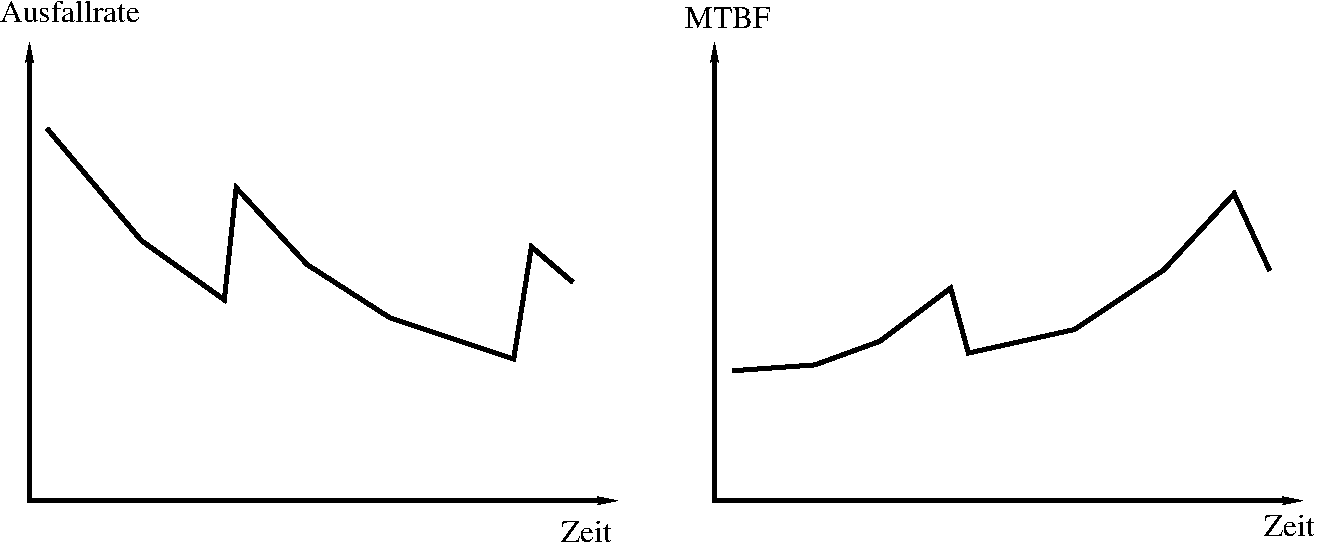
\includegraphics[width=0.8\linewidth]{lifecycle/xfig/failurerate}\\
\ifslides
{\footnotesize
\fi
\begin{tabularx}{\linewidth}{lX}
failure & Deviation of the operating behavior from its requirements \\
fault, bug & Cause of one or more malfunctions \\
error & wrong, incorrect or incomplete implementation \\
reliability & Probability of trouble-free operation during a certain period of time \\
availability & Ratio of the trouble-free operating time to the total operating time \\
\end{tabularx}
\ifslides
}
\fi
\begin{minipage}[t]{0.3\linewidth}
\small
\begin{tabular}{ll}
MTBF & mean time\\
     & between  failures\\
MTTR & mean time\\
     & to repair \\
MTTF & mean time\\
     & to failure\\
\end{tabular}

\end{minipage}
\hfill
\begin{minipage}{0.6\linewidth}
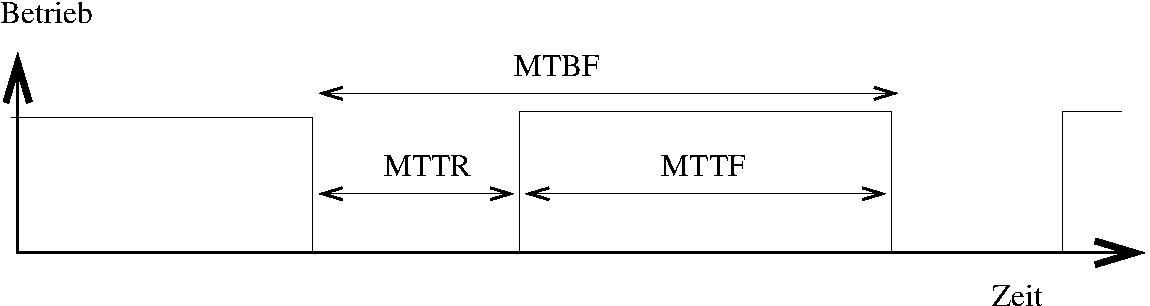
\includegraphics[width=\linewidth]{lifecycle/xfig/mttf-mttr}

{\small
\begin{tabular}{llll}
Nines of     &            \multicolumn{3}{c}{downtime per year}\\
Reliability: &         [h]    &     [min]   &     [sec]\\
\hline
2 9's (99\%)     &  87.6    &   5256.0   &  315360.0 \\
3 9's (99.9\%)    &  8.76   &    525.6   &   31536.0 \\
4 9's (99.99\%)   &  0.876  &     52.56  &    3153.6 \\
%5 9's (99.999%)   & 0.0876   &    5.256  &    315.36\\
%6 9's (99.9999%)   0.00876      0.5256      31.536
%7 9's (99.99999%)  8.76E-4      0.05256      3.1536
%
\end{tabular}
}
\end{minipage}
%
\newpage

\section{Excercise}

\begin{enumerate}
\item What is the critical path for the given task list and what is the duration (of the critical path)?
\begin{tabular}{l|l|l}
Task & Duration (Days) & Predecessor\\
\hline
A & 4 & - (Start)\\
B & 3 & A\\
C & 1 & B\\
D & 5 & - (Start)\\
E & 4 & D\\
F & 6 & E\\
G (end) & 2 & C,F\\
H & 4 & D\\
I (end) & 2 & H
\end{tabular}

\item VLC is a popular video player software. Try to find out how many lines
of code are needed based on the given user interface:\\
\vspace{3mm}
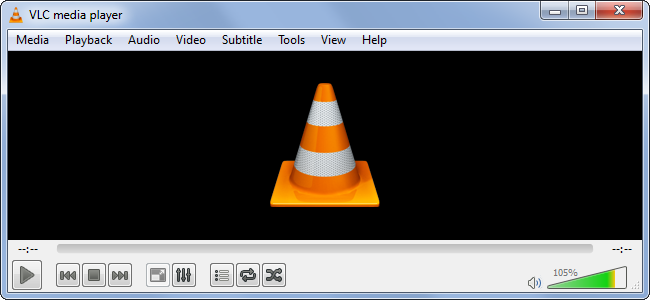
\includegraphics[width=\linewidth]{lifecycle/img/vlc}

\item You are responsible to find out how many person months are needed to
create a simple time recording software. The requirements are the following:

\begin{itemize}
\item The system is a single user system
\item A database is used to store the information
\item The user could add, delete or change an entry
\item An entry contains \emph{date, time, task}
\item A report could be created for a given month. This report will list
a activities for the specified month.
\end{itemize}

\end{enumerate}
